\begin{figure}[h]
    \centering
    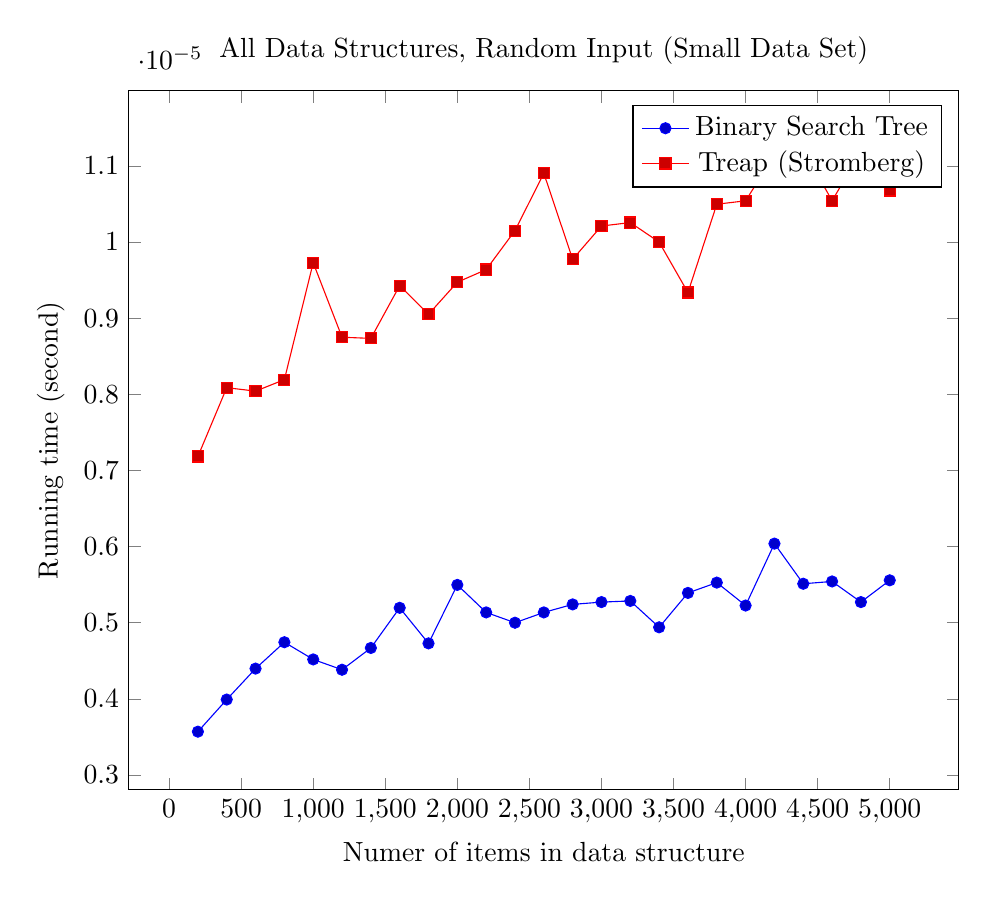
\begin{tikzpicture}
        \begin{axis}[
            xlabel={Numer of items in data structure},
            ylabel={Running time (second)},
            title={All Data Structures, Random Input (Small Data Set)},
            width=\textwidth
        ]
		\addplot coordinates {
			(200, 3.568927740493777e-06)
			(400, 3.990573211964943e-06)
			(600, 4.397159916580406e-06)
			(800, 4.743511553861879e-06)
			(1000, 4.517630051292798e-06)
			(1200, 4.382101149724704e-06)
			(1400, 4.668217719672185e-06)
			(1600, 5.195274558955631e-06)
			(1800, 4.728452787006176e-06)
			(2000, 5.496449895714406e-06)
			(2200, 5.13503949162164e-06)
			(2400, 4.999510590053547e-06)
			(2600, 5.13503949162164e-06)
			(2800, 5.2404508594783294e-06)
			(3000, 5.2705683931453254e-06)
			(3200, 5.2856271600010276e-06)
			(3400, 4.939275522719555e-06)
			(3600, 5.391038527857717e-06)
			(3800, 5.52656742942581e-06)
			(4000, 5.225392092622627e-06)
			(4200, 6.0385655018535545e-06)
			(4400, 5.511508662570108e-06)
			(4600, 5.541626196237104e-06)
			(4800, 5.2705683931453254e-06)
			(5000, 5.556684963092806e-06)
		};
		\addplot coordinates {
			(200, 7.1830317815102515e-06)
			(400, 8.086557791786576e-06)
			(600, 8.041381491263877e-06)
			(800, 8.191969159643265e-06)
			(1000, 9.727963377104131e-06)
			(1200, 8.749143532638115e-06)
			(1400, 8.734084765826822e-06)
			(1600, 9.426788040300948e-06)
			(1800, 9.05031886939689e-06)
			(2000, 9.471964340868055e-06)
			(2200, 9.637610776058737e-06)
			(2400, 1.0149608848530888e-05)
			(2600, 1.0902547190383416e-05)
			(2800, 9.77313967762683e-06)
			(3000, 1.020984391586488e-05)
			(3200, 1.0255020216387577e-05)
			(3400, 9.999021180151502e-06)
			(3600, 9.336435439299962e-06)
			(3800, 1.0495960485812362e-05)
			(4000, 1.0541136786290651e-05)
			(4200, 1.1143487459808199e-05)
			(4400, 1.1218781293997892e-05)
			(4600, 1.0541136786335059e-05)
			(4800, 1.1188663760330898e-05)
			(5000, 1.0676665687814334e-05)
		};
        \legend{Binary Search Tree, Treap (Stromberg)}
        \end{axis}
    \end{tikzpicture}
    \caption{Average of 20 operations, benchmarked every 200, starting at 200.}
\end{figure}